% Chapter 5 describes the implemented methods and their design rationale.
% Content: newline-only evaluation target, method definitions for Methods 1--5 and NNTP,
% OCR/HTR generation pipeline, and implementation safeguards.

\chapter{Methods}
\label{cha:method}

\section{Scope and Contribution Framing}
\label{sec:method_scope}

This chapter provides the methodological overview for the thesis task. The starting point is the same throughout: Historical transcriptions may already provide the character sequence, but scholarly reuse still requires recovering the line structure. The newline-only formulation isolates that problem by holding the non-newline character sequence fixed and asking where line boundaries should be inserted. The methodological description therefore specifies how the formal task from \autoref{sec:theory_problem_definition} is instantiated as evaluated alignment regimes in the sense defined in Chapter~\ref{cha:introduction}: Which evidence each configuration sees, which output constraint it is asked to satisfy, which evaluated LLM/VLM configurations instantiate the benchmark, and which recovery steps belong to the scored setup. Exact template identifiers, prompt-template/source mappings, and run-configuration details are deferred to Appendix~\ref{cha:appendix_audit} and the companion implementation repository.\footnote{Implementation provenance: \url{https://github.com/dennis-berger/llm-line-alignment}}

At the method level, the contribution has three parts: A shared newline-only transcription-alignment target, a set of LLM/VLM-based methods whose evaluated configurations vary along two design dimensions, and the deterministic baseline (NNTP) evaluated with the same downstream metric family. The five LLM/VLM-based methods are referred to as Method 1 to Method 5 (M1--M5). Their configurations are organized over two design questions: Which input evidence can support boundary placement, and how far the system should constrain, validate, repair, or project the model output before scoring \thesiscite{geng2023grammar}. The deterministic baseline is included because Connectionist Temporal Classification (CTC) transcription alignment is a close forced-alignment analogue of the thesis task: It preserves a supplied transcription and searches for line-boundary placements using recognizer-derived evidence rather than prompting a model to produce a fresh transcription \thesiscite{fischer2011icdarInaccurateAlignment,hassner2013ocrFreeAlignment,peer2025ctcBullingerAlignment}. This framing makes it possible to compare LLM/VLM-based configurations and deterministic alignment under one task scope while still keeping their setup differences explicit.

\section{Shared Transcription-Alignment Target}
\label{sec:method_common_contract}

For M1--M5, the prediction target is always the same: Recover line boundaries in a supplied transcription without changing the underlying character sequence. The fixed transcription is therefore the only admissible character source, and the LLM/VLM-based methods are designed to place newline boundaries rather than to generate new lexical content. This is the methodological move that separates line-structure recovery from recognition quality.

The evaluation target is shared, but the enforcement strength is method-dependent and part of the evaluated configuration. M1--M3 rely on prompt instructions alone and score the raw returned text directly. M4 and M5 instead ask for strict JSON of the form \texttt{\{"lines": [...]\}}, validate the returned array after generation, and, depending on the configuration, enter bounded repair, recovery, or fallback paths when the output is malformed or structurally implausible. In relation to prior work on constrained structure recovery and alignment \thesiscite{geng2023grammar,fischer2011icdarInaccurateAlignment}, the reported thesis mechanism is specifically parser-side validation plus repair rather than provider-side grammar-constrained decoding; the implemented control path is summarized in Algorithm~\ref{alg:method_structured_post_correction} and expanded in \autoref{sec:appendix_structured_pseudocode}.

For M4 and M5, exact-character preservation is achieved through boundary projection rather than by trusting copied model text. The implementation keeps the predicted line-boundary plan, maps those boundaries from the hinted text back onto the untouched supplied transcription, and stores the projected boundary plan for evaluation. Repair, method-specific recovery, fallback, and projection are therefore part of the evaluated configuration for M4 and M5 rather than a post-hoc clean-up layer outside scoring; this implementation-specific output-control path is recorded in Table~\ref{tab:method_prompt_contract} and \autoref{sec:appendix_structured_audit}.

All LLM/VLM-based configurations are evaluated by the shared metric stack from \autoref{sec:experimentation_line_alignment_metrics}. NNTP is evaluated with the same downstream metrics, but its preparation stage normalizes and filters labels to the active PyLaia symbol inventory before alignment. The shared evaluation is therefore strong at the metric level, especially for line-boundary outcomes, yet not perfectly identical at the character-inventory level.

The method scope is handwritten-first. M1--M5 form the main handwritten evaluation on the four handwritten datasets, while Bullinger Print and IAM Print are reported as secondary printed context. The focused print evaluation covers M1--M3 rather than the line-image and structured-output configurations, so it should not be read as evidence for the full M1--M5 method set.

\paragraph{Prompt design principles.}
\label{sec:method_prompt_principles}

Table~\ref{tab:method_prompt_contract} summarizes the thesis-level prompt requirements shared by the LLM/VLM-based method set. It describes the scientific intent of the prompts rather than reproducing their full wording. Exact implementation identifiers, prompt-template/source mappings, and run-configuration details are listed in \autoref{sec:appendix_prompt_templates}.

\begin{table}[H]
  \centering
  \caption{Compact schematic prompt requirements for the LLM/VLM-based method set.}
  \label{tab:method_prompt_contract}
  \small
  \renewcommand{\arraystretch}{1.08}
  \begin{tabularx}{\linewidth}{@{}p{0.25\linewidth}Y@{}}
    \toprule
    \textbf{Aspect} & \textbf{Requirement} \\
    \midrule
    Character source & The supplied transcription is the only admissible source of characters. \\
    Allowed edit & Only newline boundaries may be inserted; the character sequence itself must remain fixed. \\
    Normalization & No spelling correction, modernization, normalization, or semantic rewriting is allowed. \\
    OCR/HTR evidence & OCR/HTR is used only as structural evidence about likely boundaries and reading order, never as replacement text. \\
    Structured output (M4/M5) & The response must be strict JSON with exactly \(N\) lines, where \(N\) is the expected line count supplied by the evaluated configuration. \\
    Failure handling (M4/M5) & If the strict JSON requirement fails, the configuration may attempt one repair pass, method-specific recovery from model lines, or deterministic fallback before final projection to the supplied transcription. \\
    \bottomrule
  \end{tabularx}
\end{table}

The requirements in Table~\ref{tab:method_prompt_contract} also clarify the main asymmetry inside M1--M5. M1--M3 depend entirely on whether the initial prompt is followed faithfully, whereas M4 and M5 score a controlled boundary plan after validation and, when needed, recovery. This distinction belongs to the method definition itself: Later comparisons inherit a shared target, but not identical output-control strength.

\section{Method Set Overview}
\label{sec:method_overview}

With the newline-only constraint fixed, the method set is organised by two design axes rather than by a single incremental ladder. The first axis is \emph{input evidence}: Page images, OCR/HTR text, ordered OCR-line metadata, ordered line crops, and recognizer observations each expose different boundary cues. The second axis is \emph{output control}: Raw returned text, structured JSON validation, repair or fallback, projection to the supplied transcription, and deterministic forced alignment make different commitments about how a candidate boundary plan becomes the scored object. The overview tables and figures therefore introduce a design space before the individual method descriptions supply operational detail.

Intuitively, M1--M3 ask how much boundary evidence remains useful under weak output control, where the raw returned text is scored directly. M4--M5 test structured output control together with richer line-level evidence, so the evaluated object is a projected boundary plan selected from accepted, repaired, recovered, or fallback hints. NNTP then provides a deterministic forced-alignment anchor rather than another prompted generation configuration.

\begin{table}[t]
  \centering
  \caption{Method-set overview for the implemented configurations. M1--M5 share the newline-only target but vary along the evidence and output-control dimensions; NNTP is the deterministic baseline evaluated with the same downstream metric family but with PyLaia-filtered labels.}
  \label{tab:method_regime_comparison}
  \small
  \renewcommand{\arraystretch}{1.08}
  \setlength{\tabcolsep}{4pt}
  \begin{tabularx}{\linewidth}{@{}>{\raggedright\arraybackslash}p{0.18\linewidth}>{\raggedright\arraybackslash}p{0.11\linewidth}>{\raggedright\arraybackslash}p{0.23\linewidth}>{\raggedright\arraybackslash}p{0.20\linewidth}>{\raggedright\arraybackslash}X@{}}
    \toprule
    \textbf{Configuration family} & \textbf{Methods} & \textbf{Input evidence} & \textbf{Output control} & \textbf{Purpose in the thesis} \\
    \midrule
    Raw LLM/VLM output regimes & M1--M3 & Supplied transcription plus page images, \OCRHTR text, or both, depending on the concrete configuration & Prompt instructions only; raw returned text is scored directly & Tests how much boundary structure can be recovered by changing the evidence supplied to an otherwise raw-output configuration \\
    Structured LLM/VLM regimes & M4--M5 & Supplied transcription plus ordered OCR-line metadata or ordered line-image crops; the evaluated M5 configuration also supplies OCR/HTR line text and page-level context & Strict JSON, parser validation, one repair pass, method-specific fallback or recovery, and projection to the supplied transcription & Tests whether stronger output-control paths and line-level anchors reduce character drift and boundary ambiguity \\
    Deterministic baseline & NNTP & Fixed transcription, ordered line-image evidence, and recognizer-derived CTC observations & Deterministic forced alignment over labels filtered to the active PyLaia symbol inventory & Provides a non-prompt comparison for the same newline-boundary metric family while keeping the symbol-filtering caveat explicit \\
    \bottomrule
  \end{tabularx}
\end{table}

The key comparison axis in \autoref{tab:method_regime_comparison} combines which modality is present with how strongly structure is anchored and how strongly outputs are controlled afterward. M1--M3 isolate evidence choices inside a raw LLM/VLM output configuration; M4--M5 combine line-level evidence with structured response validation and projection; NNTP replaces generative prompting with deterministic forced alignment over recognizer observations. The table should therefore be read as an inventory of implemented configurations, not as a ladder in which a single factor changes at a time.

\begin{table}[H]
  \centering
  \caption{Compact method cards for the implemented regimes. The table keeps the main-text interpretation variables; \autoref{sec:appendix_method_comparability} expands them into the appendix comparability registry.}
  \label{tab:method_comparability_matrix}
  \scriptsize
  \renewcommand{\arraystretch}{1.06}
  \setlength{\tabcolsep}{2pt}
  \begin{tabularx}{\linewidth}{@{}>{\raggedright\arraybackslash}p{0.055\linewidth}*{7}{>{\raggedright\arraybackslash}X}@{}}
    \toprule
    \textbf{Method} & \textbf{Input evidence} & \textbf{Expected line-count source} & \textbf{Output type} & \textbf{Validation/repair} & \textbf{Projection/\allowbreak fallback} & \textbf{Scored object} & \textbf{Main caveat} \\
    \midrule
    M1 & page image(s) + fixed transcription & none; count emerges & line-broken text & prompt only & none & raw returned text & heuristic page chunking \\
    M2 & page image(s) + \OCRHTR{} hint + fixed transcription & none; count emerges & line-broken text & prompt only & none & raw returned text & OCR noise + chunking \\
    M3 & \OCRHTR{} hint + fixed transcription & none; count emerges & line-broken text & prompt only & none & raw returned text & no visual correction \\
    M4 & ordered OCR-line scaffold + expected \(N\) + fixed transcription & stored \texttt{ocr\_lines} count & JSON line list & parse; exact \(N\); one repair & project accepted or fallback plan & projected boundary plan & known count; OCR scaffold \\
    M5 & ordered line crops + \OCRHTR{} line text + page context + expected \(N\) + fixed transcription & stored \texttt{ocr\_lines} count & JSON line list & parse; exact \(N\); repair/checks & recovery or fallback; projection & projected boundary plan & heterogeneous crop provenance; image-packaging limits \\
    NNTP & line images + recognizer output + fixed transcription & staged line-image set & forced-alignment reconstruction & deterministic checks & not applicable & filtered reconstruction & PyLaia symbol-inventory filter \\
    \bottomrule
  \end{tabularx}
\par\vspace{0.35em}
  \parbox{0.98\linewidth}{\footnotesize\raggedright \textit{Note.} The caveat column is intentionally compact. Table~\ref{tab:method_line_evidence_sources} consolidates the known-count and crop-provenance caveats for M4/M5, while \autoref{sec:method_safeguards_limits} collects the cross-method interpretation limits, including backend image-packaging limits and NNTP's PyLaia-side symbol filtering.}
\end{table}

\paragraph{What is scored?}
M1--M3 score raw returned text: Copied-character changes, omissions, normalizations, or extra prose remain part of the prediction. M4 and M5 score projected boundary plans selected from accepted, repaired, recovered, or fallback hints. NNTP scores deterministic reconstruction after PyLaia-side filtering. This is the same scored-object distinction used by the Chapter~\ref{cha:experimentation} output-control analysis.

Figures~\ref{fig:method_regime_ladder} and~\ref{fig:method_pipeline_overview} split that overview into two readable views. The first marks the boundary between raw-output M1--M3 and structured M4/M5, while the second isolates the shared structured-control skeleton from stored ordered line metadata to evaluation. Dataset-specific crop provenance stays in Table~\ref{tab:method_line_evidence_sources}, while \autoref{sec:appendix_structured_audit} holds the fuller structured-control tables used later for traceability.

\begin{figure}[H]
  \centering
  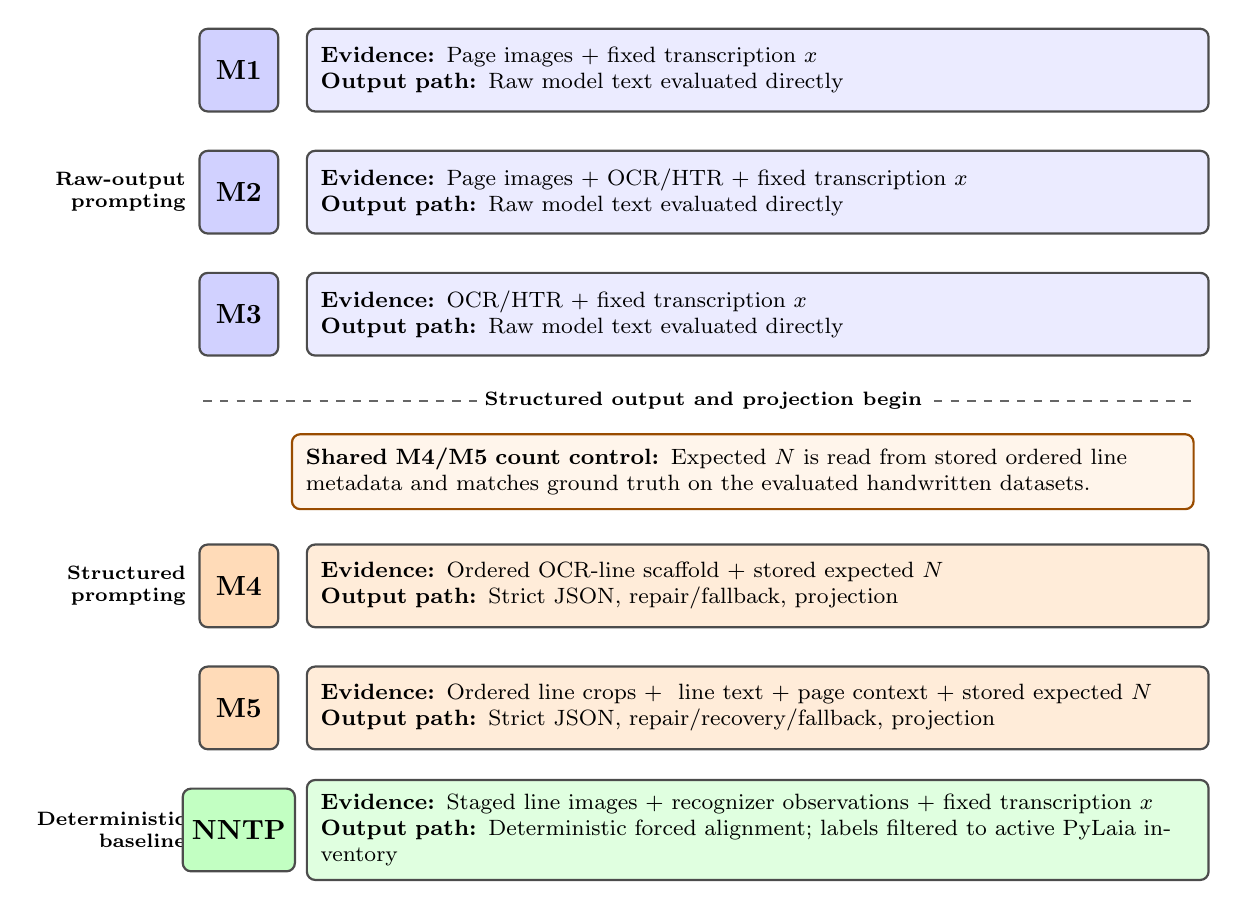
\begin{tikzpicture}[
    x=1cm,
    y=1cm,
    font=\footnotesize,
    method/.style={rectangle, rounded corners=3pt, draw=black!70, thick, align=left, text width=11.1cm, minimum height=1.05cm, inner sep=5pt},
    raw/.style={method, fill=blue!8},
    structured/.style={method, fill=orange!15},
    baseline/.style={method, fill=green!12},
    tag/.style={rectangle, rounded corners=3pt, draw=black!70, thick, minimum width=1.0cm, minimum height=1.05cm, font=\bfseries},
    note/.style={rectangle, rounded corners=3pt, draw=orange!60!black, thick, fill=orange!8, align=left, text width=11.1cm, inner sep=5pt}
  ]
    \node[tag, fill=blue!18] (m1tag) at (0,0) {M1};
    \node[raw, anchor=west] (m1) at (0.85,0) {\textbf{Evidence:} Page images + fixed transcription \(x\)\\\textbf{Output path:} Raw model text evaluated directly};

    \node[tag, fill=blue!18] (m2tag) at (0,-1.55) {M2};
    \node[raw, anchor=west] (m2) at (0.85,-1.55) {\textbf{Evidence:} Page images + OCR/HTR + fixed transcription \(x\)\\\textbf{Output path:} Raw model text evaluated directly};

    \node[tag, fill=blue!18] (m3tag) at (0,-3.10) {M3};
    \node[raw, anchor=west] (m3) at (0.85,-3.10) {\textbf{Evidence:} OCR/HTR + fixed transcription \(x\)\\\textbf{Output path:} Raw model text evaluated directly};

    \draw[black!60, dashed, line width=0.9pt] (-0.45,-4.20) -- (12.20,-4.20);
    \node[fill=white, inner sep=2pt, font=\scriptsize\bfseries] at (5.90,-4.20) {Structured output and projection begin};
    \node[anchor=east, align=right, font=\scriptsize\bfseries] at (-0.55,-1.55) {Raw-output\\prompting};

    \node[note] (sharednote) at (6.40,-5.10) {\textbf{Shared M4/M5 count control:} Expected \(N\) is read from stored ordered line metadata and matches ground truth on the evaluated handwritten datasets.};
    \node[anchor=east, align=right, font=\scriptsize\bfseries] at (-0.55,-6.55) {Structured\\prompting};

    \node[tag, fill=orange!28] (m4tag) at (0,-6.55) {M4};
    \node[structured, anchor=west] (m4) at (0.85,-6.55) {\textbf{Evidence:} Ordered OCR-line scaffold + stored expected \(N\)\\\textbf{Output path:} Strict JSON, repair/fallback, projection};

    \node[tag, fill=orange!28] (m5tag) at (0,-8.10) {M5};
    \node[structured, anchor=west] (m5) at (0.85,-8.10) {\textbf{Evidence:} Ordered line crops + \OCRHTR{} line text + page context + stored expected \(N\)\\\textbf{Output path:} Strict JSON, repair/recovery/fallback, projection};

    \node[anchor=east, align=right, font=\scriptsize\bfseries] at (-0.55,-9.65) {Deterministic\\baseline};
    \node[tag, fill=green!24] (nntptag) at (0,-9.65) {NNTP};
    \node[baseline, anchor=west] (nntp) at (0.85,-9.65) {\textbf{Evidence:} Staged line images + recognizer observations + fixed transcription \(x\)\\\textbf{Output path:} Deterministic forced alignment; labels filtered to active PyLaia inventory};
  \end{tikzpicture}
  \caption{Evidence and output-control overview for the implemented M1--M5 configurations. The dashed divider marks the shift from raw-output prompting (M1--M3) to structured prompting with projection (M4--M5).}
  \label{fig:method_regime_ladder}
\end{figure}

\begin{figure}[H]
  \centering
  \begin{tikzpicture}[
    node distance=0.48cm,
    font=\footnotesize,
    >={Latex[length=2mm]},
    stage/.style={rectangle, rounded corners=3pt, draw=black!70, thick, align=center, text width=10.3cm, minimum height=0.95cm, inner sep=5pt},
    input/.style={stage, fill=gray!10},
    control/.style={stage, fill=orange!15},
    eval/.style={stage, fill=blue!8},
    flow/.style={->, thick}
  ]
    \node[input] (ocrjson) {stored ordered line metadata\\shared structured payload for M4/M5; M4 uses ordered OCR-line hints and evaluated M5 resolves ordered line crops plus \OCRHTR{} line text and page context};
    \node[input, below=of ocrjson] (count) {expected \(N\) read from stored metadata\\matches ground truth on the evaluated handwritten datasets};
    \node[control, below=of count] (strict) {strict JSON response\\\texttt{\{"lines": ["...", "..."]\}}};
    \node[control, below=of strict] (repair) {one repair prompt if the JSON is malformed or has the wrong line count};
    \node[control, below=of repair] (fallback) {recovery or deterministic fallback after the strict path fails\\(M5 may reconcile loose response lines; M4 falls back deterministically)};
    \node[control, below=of fallback] (projection) {projection of the selected boundary plan back onto the untouched transcription \(x\)};
    \node[eval, below=of projection] (evaluation) {evaluation\\line accuracy, exact-line precision/recall/F1, raw/normalized CER/WER};

    \draw[flow] (ocrjson) -- (count);
    \draw[flow] (count) -- (strict);
    \draw[flow] (strict) -- (repair);
    \draw[flow] (repair) -- (fallback);
    \draw[flow] (fallback) -- (projection);
    \draw[flow] (projection) -- (evaluation);
  \end{tikzpicture}
  \caption{Structured-output control skeleton for M4 and M5. Raw-output methods M1--M3 are excluded because they do not pass through known-count staging, JSON validation, repair/fallback, and projection; M5 additionally includes recovery and page-wise subdivision for long inputs.}
  \label{fig:method_pipeline_overview}
\end{figure}

\FloatBarrier

\section{Benchmarked LLM/VLM Model Families and Capabilities}
\label{sec:method_benchmarked_models}

The LLM/VLM part of the benchmark uses contemporary general-purpose multimodal model families rather than task-specific handwriting recognizers or dedicated transcript-alignment models. The relevant capability is not only visual recognition. For newline-only alignment, a model must be able to receive document-image evidence and textual context, follow instructions about a fixed transcription, and return either line-broken text or a structured representation that can later be validated and projected back to the supplied transcription. This section records the model families and capabilities needed to interpret the benchmark \thesiscite{openai2026gpt54,openai2026models,google2026geminiModels,google2026gemini25Models,bai2025qwen3vl,mistral2026models,mistral2026vision}.

\paragraph{OpenAI GPT configurations.}
The OpenAI configurations are hosted multimodal LLM/VLM systems used through an API backend. In the thesis artifacts they are represented by the display names GPT-5.4-0305 and GPT-5.2. The important capability for this work is that these configurations support text interaction together with image input, so they can be prompted with a fixed transcription plus page or line-image evidence. GPT-5.4-0305 is treated as the main OpenAI configuration in the benchmark, while GPT-5.2 is retained as an earlier OpenAI configuration for historical and diagnostic context. The display names used in the thesis refer to the archived provider identifiers recorded in Appendix Table~\ref{tab:app_model_provider_aliases}, not to later model versions or later provider behavior \thesiscite{openai2026gpt54,openai2026models}.

\paragraph{Google Gemini configurations.}
The Gemini configurations represent Google's hosted multimodal model family. They are included because the task requires a general-purpose model that can combine visual document evidence with textual instructions and \OCRHTR{}-derived context. In this thesis, Gemini rows are used as additional provider evidence rather than as an architectural study of the Gemini family. The exact Gemini display names, provider identifiers, and retained experiment rows are documented in Appendix Table~\ref{tab:app_model_provider_aliases} \thesiscite{google2026geminiModels,google2026gemini25Models}.

\paragraph{Qwen3-VL configurations.}
Qwen3-VL represents a vision-language instruction-model family with dense 8B and 32B variants documented in the cited model-family literature. In contrast to the hosted API configurations, the retained Qwen3-VL rows are executed through the Hugging Face backend and GPU-cluster job scripts. This distinction matters for reproducibility because local execution depends on model weights, hardware memory, inference settings, and job scripts rather than only on a remote API call. In the thesis, the Qwen3-VL-8B and Qwen3-VL-32B display names identify the archived evaluated variants; they should not be read as a controlled model-size ablation unless such a comparison is stated explicitly \thesiscite{bai2025qwen3vl}.

\paragraph{Mistral configuration.}
Mistral-2512 is the thesis display name for an archived Mistral Large configuration with image-input support. It is included as an additional hosted multimodal model-family check. Its role in the thesis is to broaden the evaluated model landscape beyond the OpenAI, Gemini, and Qwen3-VL families while preserving the same newline-only task definition \thesiscite{mistral2026models,mistral2026vision}.

Across all of these model families, the thesis evaluates complete alignment configurations rather than intrinsic model quality. The same model can behave differently depending on the supplied evidence, prompt format, structured-output requirements, validation, repair, fallback, and projection. NNTP is intentionally not part of this LLM/VLM model set; it is a deterministic forced-alignment baseline based on recognizer-derived CTC evidence and token passing, and is therefore described separately in \autoref{sec:method_nntp} \thesiscite{graves2006ctc,peer2025ctcBullingerAlignment}.

For exact provider identifiers, aliases, row coverage, denominator status, and notes, see Appendix Table~\ref{tab:app_model_provider_aliases}.

\FloatBarrier

\section{Source of Line-Level Evidence and Line-Count Information}
\label{sec:method_line_evidence_sources}

The structured methods need one more design clarification before they can be compared fairly. Reliable ordered line metadata is an operational prerequisite of M4/M5 as evaluated. In the handwritten datasets used here, the stored \texttt{ocr\_lines} cardinality matches the ground-truth line count for the evaluated samples. The structured configurations therefore test boundary assignment under known-count staging rather than blind line-count prediction.

Table~\ref{tab:method_line_evidence_sources} makes the corresponding artifact provenance explicit. Children and IAM use dataset-provided presegmented line images, Bullinger reuses PAGE/XML-derived line images, and Washington uses curated Kraken crops with one crop per ground-truth line. M4 consumes ordered OCR-line text derived from these assets, M5 uses the crops as local visual anchors with OCR/HTR line text as secondary context in the evaluated configuration, and NNTP consumes the same or equivalent staged line-image sets depending on dataset.

\begin{table}[H]
  \centering
  \caption{Dataset-specific line evidence and known-count source on the evaluated handwritten datasets. The table makes explicit that M4 and M5 require reliable ordered line metadata and use stored structured line cardinality as the expected line count, whereas NNTP operates on staged line-image sets whose preparation also constrains the effective line inventory.}
  \label{tab:method_line_evidence_sources}
  \footnotesize
  \renewcommand{\arraystretch}{1.08}
  \setlength{\tabcolsep}{4pt}
  \begin{tabularx}{\linewidth}{@{}>{\raggedright\arraybackslash}p{0.16\linewidth}>{\raggedright\arraybackslash}p{0.24\linewidth}>{\raggedright\arraybackslash}p{0.18\linewidth}>{\raggedright\arraybackslash}p{0.18\linewidth}>{\raggedright\arraybackslash}X@{}}
    \toprule
    \textbf{Dataset} & \textbf{Crop provenance / order} & \textbf{M4 evidence} & \textbf{M5 evidence} & \textbf{NNTP staging} \\
    \midrule
    Bullinger & PAGE/XML-derived line crops; PAGE reading order & PyLaia OCR over PAGE/XML line images & ordered PAGE/XML line crops as visual anchors; OCR/HTR line text as secondary context & PAGE/XML line images staged directly; placeholder lines filtered so the staged set matches processed ground truth \\
    Children Handwritten & dataset-provided line images; dataset line order & PyLaia OCR over dataset-provided line images & ordered dataset-provided line images as visual anchors; OCR/HTR line text as secondary context & dataset-provided line images staged directly; line-image count required to match ground truth \\
    IAM & official IAM line images; official line order & PyLaia OCR over official IAM line images & ordered official IAM line images as visual anchors; OCR/HTR line text as secondary context & official IAM line images staged directly; line-image count required to match ground truth \\
    Washington Handwritten & curated Kraken line images with one crop per ground-truth line; curated page order & PyLaia OCR over curated Kraken line images & ordered curated Kraken line images as visual anchors; OCR/HTR line text as secondary context & curated Kraken line images staged directly; final staged inventory contains one crop per ground-truth line \\
    \bottomrule
  \end{tabularx}
\par\vspace{0.35em}
  \parbox{0.98\linewidth}{\footnotesize\raggedright \textit{Notes.} This table consolidates the structured-regime evidence prerequisites. For M4 and M5, reliable ordered line metadata is an operational prerequisite, and its stored \texttt{ocr\_lines} cardinality matches the ground-truth line count in the reported evaluation set on every sample. Crop provenance differs across datasets: Bullinger uses PAGE/XML-derived crops, Children and IAM use dataset-provided line images, and Washington uses curated Kraken crops with one crop per ground-truth line.}
\end{table}

Table~\ref{tab:method_line_evidence_sources} is the main reason M4 and M5 should be read as known-count structured configurations in the evaluated handwritten datasets. They combine structural evidence, output control, and a reliable ordered-line prerequisite whose cardinality matches ground truth. The boundary of that claim is equally important: The evaluated M4/M5 rows do not test blind page-side line-count prediction.

\clearpage

\section{Raw LLM/VLM Output and Input-Evidence Regimes}
\label{sec:method_raw_prompt_output}

The first LLM/VLM-based family asks what happens when the evidence changes but output control remains deliberately weak. In this chapter, \emph{raw LLM/VLM output} means that the model is asked to return the line-broken transcription directly, and that this raw returned text is the object evaluated by the metric stack. M1--M3 therefore test input evidence rather than parser-side enforcement: M1 uses page images, M2 adds OCR/HTR text to the page images, and M3 removes images so that OCR/HTR lineation becomes the only structural cue.

\paragraph{M1: Image + transcription.}
\label{sec:method_m1}
M1 receives the ordered page-image sequence together with the full supplied transcription. For multi-page samples, the runner does not know the true page boundary in the transcription. It therefore splits the transcription into contiguous chunks of roughly equal character length, cuts only on word boundaries, assigns one chunk to each page image, skips empty chunks, runs one multimodal call per page, and concatenates the page outputs in page order.

The M1 image-transcription prompt asks the model to reconstruct line breaks from page layout alone while keeping the transcriptional character sequence fixed. Output control is entirely prompt-level. M1 has no explicit line-count constraint, no parser-backed repair loop, and no deterministic post-hoc restoration if a model copies a character span incorrectly. The configuration therefore measures how much line structure can be recovered from page images alone, but also how much the result depends on instruction following and the initial page-chunk heuristic. \autoref{sec:appendix_prompt_templates} records the template identifier and associated run-configuration details.

\paragraph{M2: Image + transcription + OCR/HTR.}
\label{sec:method_m2}
M2 keeps the M1 page-image configuration and adds \OCRHTR text as an auxiliary structural hint. Here \emph{OCR/HTR text} means machine-recognized text produced by the shared preprocessing pipeline; it is evidence about likely reading order and line breaks, not a replacement for the supplied transcription. In multi-page samples, the implementation again uses heuristic page assignment rather than true page-level alignment: It splits both the supplied transcription and the \OCRHTR text independently into roughly equal-length word-respecting chunks, pairs those chunks with the ordered page images, and runs one call per page.

The M2 image-transcription-\OCRHTR prompt is intended to use OCR/HTR as structural guidance rather than as replacement text. In practice, however, the page-local hint depends on the accuracy of the upstream segmentation or recognition and the chunking heuristic used to align it to page images. The configuration therefore tests OCR-conditioned structural evidence together with its sensitivity to upstream OCR noise and page-chunk assignment \thesiscite{marz2021dataCentricDomainAdaptation,li2023trocr}. As in M1, the raw returned text is scored directly, without parser-backed repair or projection.

\paragraph{M3: Transcription + OCR/HTR only.}
\label{sec:method_m3}
M3 removes the page image and aligns the transcription against \OCRHTR text in a single text-only call. Its inputs are the full supplied transcription and the full \OCRHTR text from the preprocessing pipeline. When the OCR pipeline has processed a multi-page sample, page texts are already concatenated in order with blank-line page separation, and M3 consumes that combined text as-is rather than re-splitting it by page.

The M3 transcription-\OCRHTR prompt uses OCR/HTR lineation as its only structural cue. Because M3 has no direct visual evidence, it avoids image-side ambiguity but cannot correct layout cues that are absent from the OCR text. Like M1 and M2, it remains a raw-output configuration at evaluation time. This makes M3 the main OCR-conditioned raw-output comparator among the LLM/VLM-based methods.

\section{Structured LLM/VLM Regimes and Post-Correction}
\label{sec:method_structured_regimes}

The second LLM/VLM-based family keeps the newline-only target but changes the control dimension. M4 and M5 still ask an LLM or VLM to infer line boundaries, but they do not score copied model text as final output. A \emph{structured LLM/VLM regime} means that the response must be strict JSON of the form \texttt{\{"lines": [...]\}}, the parser checks that the array has the expected line count, and the selected boundary plan is projected back onto the untouched supplied transcription before evaluation. In this context, \emph{post-correction} denotes the bounded repair, recovery, fallback, and projection steps that are part of the evaluated configuration, not an unscored manual clean-up step.

Implementation-wise, projection treats accepted, recovered, or fallback line strings as boundary hints rather than final content. The helper concatenates those hint strings, records the cumulative offsets between hinted lines, maps those offsets onto the supplied transcription with monotonic \texttt{SequenceMatcher} anchors and interpolation between anchors, and then re-slices the untouched transcription at the projected offsets. Copied-character drift in a structured response is therefore not retained in the scored output; remaining differences are boundary-placement differences under the selected plan. If strict JSON and the repair attempt fail, M4 falls back to OCR hint lines, while M5 first tries loose JSON reconciliation against OCR hint lines and otherwise uses OCR or exact-count response-line fallback before projection, raising an error if no usable line hints remain.

Algorithm~\ref{alg:method_structured_post_correction} gives the main-text version of this control path. The model is not trusted to author the final transcription directly: It supplies a candidate line plan under a strict JSON requirement, and the pipeline accepts that plan only after structural validation. If the response is malformed or has the wrong number of lines, the pipeline may try one repair prompt; if no valid model plan remains, the implementation uses method-specific recovery or fallback paths derived from ordered line evidence where available. The selected line plan is then projected back onto the untouched transcription \(x\), so the scored output preserves the original non-newline character sequence and differs only in boundary placement.

\begin{algorithm}[htbp]
  \caption{Concise structured post-correction pipeline for M4/M5.}
  \label{alg:method_structured_post_correction}
  \begin{minipage}{0.96\linewidth}
    \footnotesize
\begin{alltt}
Input: Untouched transcription x; ordered evidence e; method M in \{M4,M5\}
1. load untouched transcription x
2. load ordered evidence e
3. read expected line count N from e
4. build the structured prompt from x, e, N, and M
5. call the model
6. parse the response as strict JSON with a "lines" array
7. validate that the array contains exactly N strings
8. if validation fails and repair is enabled, attempt one repair call
9. for M5, optionally check accepted plans for structural/quality faults
10. if no valid plan is accepted, use deterministic fallback when available
11. select the final boundary plan and project it back onto untouched x
12. score the newline-only output with the shared metric stack
\end{alltt}
  \end{minipage}
\end{algorithm}

This compact algorithm is intentionally shorter than the appendix version. \autoref{sec:appendix_structured_pseudocode} keeps method-specific details such as M5 line-image resolution, loose recovery from malformed response lines, post-validation structural and quality checks, page-wise subdivision for long inputs, candidate-plan selection, and trace-level resolution modes. The Chapter~5 algorithm instead marks the conceptual difference from raw prompting: M4 and M5 evaluate structured, validated, and projected boundary plans, whereas M1--M3 evaluate the raw returned transcription. Chapter~\ref{cha:experimentation} later interprets those configurations rather than treating repair, fallback, projection, or M5-specific quality checks as separately ablated components.

\paragraph{M4: Structured OCR-line alignment.}
\label{sec:method_m4}
M4 takes the supplied transcription together with an ordered OCR-line record rather than a plain OCR text file. Each hint line carries reading-order information and OCR text, and the evaluated handwritten configuration uses that stored record in four coupled steps: The expected line count \(N\) is read from the stored record, the M4 structured OCR-line prompt is required to return strict JSON with exactly \(N\) strings, one repair prompt is allowed after a failed first parse, and any accepted or fallback boundary plan is projected back onto the untouched transcription before scoring. The dataset-specific source and ground-truth relation of that expected count are consolidated in \autoref{tab:method_line_evidence_sources}.

The reported M4 path is parser-validated rather than grammar-constrained. A malformed response triggers one repair attempt; if the strict path still fails, the implementation falls back to deterministic projection from the ordered OCR hints. Even successful JSON is not trusted as a character string in its own right: Copied-character drift is removed during final projection, so the stored output preserves the boundary plan rather than copied model characters. Stored \(N\), one-repair control, deterministic fallback, and final projection are therefore part of the evaluated M4 configuration rather than minor implementation details; Algorithm~\ref{alg:method_structured_post_correction} and \autoref{sec:appendix_structured_pseudocode} record the implemented control path.

M4 therefore moves the task from page-level prompting toward alignment against an explicit ordered scaffold. Its configured role is stronger structural control and exact-character preservation after projection. The relevant interpretation boundaries are the OCR scaffold and the known-count provenance summarized in \autoref{tab:method_line_evidence_sources}; these combine the general problem of OCR-conditioned downstream behavior \thesiscite{marz2021dataCentricDomainAdaptation} with the thesis-specific known-count setup. \autoref{sec:appendix_prompt_templates} and \autoref{sec:appendix_structured_pseudocode} record the implementation identifiers and control-path pseudocode.

\paragraph{M5: Context-grounded line-image alignment.}
\label{sec:method_m5}
M5 uses ordered line-image crops as its primary structural signal. It consumes the supplied transcription together with the same structured line metadata used by M4, resolves ordered line crops from that record, and, in the evaluated M5 configuration, exposes OCR/HTR line text and page-level context as secondary evidence. The resulting setup is a context-rich line-image regime: Local crop evidence is primary, OCR/HTR is auxiliary, and page context is available to reduce long-range drift rather than to replace local anchors. The dataset-specific source of those anchors is consolidated in \autoref{tab:method_line_evidence_sources}.

The evaluated M5 configuration begins with the same strict-JSON output-validity requirement and one-repair pattern as M4, but the configuration is broader than a single parse-or-repair loop. Operationally, recovery means extracting a plausible ordered line list from malformed or wrong-count responses, reconciling it against the expected line count and stored line structure, retrying page-local subproblems for long inputs, and falling back to deterministic boundary allocation when no usable model plan remains. In addition, an exact-count JSON response is not necessarily the final boundary plan: The evaluated M5 path may still check for structural symptoms such as implausibly short standalone lines, use OCR/HTR-backed quality repair when the selected plan is weak against the ordered hints, and select among candidate projected plans before storing the final newline-only output. As with M4, the known-count staging, repair, recovery, quality checks, fallback, candidate selection, and projection are part of the scored configuration rather than post-hoc clean-up. \autoref{sec:appendix_structured_audit} summarizes these branches, while Table~\ref{tab:app_m5_trace_event_counts} reports which resolution modes are preserved in the available trace records.

Because M5 packages many images, the concrete prompt bundle is still backend-conditioned. The evaluated M5 configuration requests rich local and global visual context, but runtime packaging may be reduced to fit backend image limits or page-boundary constraints. This configuration should be interpreted as a combined evidence-and-control setup. It does not isolate line images, OCR/HTR line text, page context, one architecture, or output control as independent components. Further run-configuration details for the zero-shot context-rich M5 configuration are documented in Table~\ref{tab:method_m5_context_rich_config}.

\section{Deterministic Baseline (NNTP)}
\label{sec:method_nntp}

The deterministic baseline (NNTP) is used here as the public LSTM-RNN token-passing / forced-alignment implementation associated with the Bullinger alignment study. This thesis does not reimplement NNTP from scratch. It uses the public NNTP implementation released with that study and adapts the surrounding preparation and evaluation scripts to the thesis artifact representation.\footnote{Implementation provenance: \url{https://github.com/andreas-fischer-unifr/nntp}, accessed 8 May 2026. This GitHub repository is cited here as a provenance pointer for the baseline implementation, not as a scholarly bibliography source.} NNTP is not an LLM/VLM-based method and it does not freely generate a new transcription. Instead, it takes a fixed transcription, ordered line-image evidence, and recognizer-derived CTC observations, then searches for the alignment path that places the fixed character sequence against those observations and recovers newline boundaries. This makes NNTP a deterministic baseline for newline-only boundary reconstruction, but one with different evidence requirements from M1--M5 \thesiscite{graves2006ctc,peer2025ctcBullingerAlignment}.

Operationally, the thesis-side NNTP pipeline has five stages: Preparation, recognizer netout generation, lattice conversion, forced alignment, and evaluation. The pipeline can start either from PAGE/XML geometry or from datasets that already provide ordered line-image sets. For fixed staged inputs, recognizer outputs, symbol inventory, and implementation tie-handling, the forced-alignment stage is deterministic: Repeated decoding follows the same scored alignment path rather than sampling a language-model response \thesiscite{fischer2011icdarInaccurateAlignment,peer2025ctcBullingerAlignment}.

\begin{algorithm}[htbp]
  \caption{Concise NNTP forced-alignment pipeline.}
  \label{alg:method_nntp_pipeline}
  \begin{minipage}{0.96\linewidth}
    \footnotesize
\begin{alltt}
Input: Fixed x; ordered line-image evidence g; active PyLaia symbol inventory S
1. prepare ordered line images g
2. normalize and filter x to labels present in S
3. generate recognizer netouts / CTC observations for g
4. convert lattices or observations and construct boundary maps
5. run deterministic forced alignment over the filtered label sequence
6. reconstruct newline boundaries from the aligned observation path
7. evaluate the resulting line breaks with the shared metric stack
\end{alltt}
  \end{minipage}
\end{algorithm}

NNTP filters labels to the active PyLaia symbol inventory before forced alignment; Appendix~\ref{sec:appendix_nntp_symbol_filter_audit} audits the archived support for this preprocessing step. Later conversion, alignment, reconstruction, and evaluation operate on that filtered label sequence. This preserves NNTP's role as a fixed-transcription forced aligner rather than an LLM/VLM method, and character-level comparisons against M1--M5 therefore retain the filtering boundary collected again in \autoref{sec:method_safeguards_limits} \thesiscite{graves2006ctc,peer2025ctcBullingerAlignment}.

The preparation rules differ by dataset type. PAGE/XML datasets derive page and line order from XML reading-order metadata, crop ordered line images from the page geometry, and skip structural placeholder lines that are not part of the text content. Presegmented datasets stage the existing line-image folders directly, require the line-image count to match the ground-truth line count, and use the existing ground-truth line order as the target sequence for boundary reconstruction. After preparation, PyLaia netout produces CTC lattices, the conversion stage rewrites them into observation files plus boundary maps, and the NNTP aligner forces the filtered label sequence against those observations to reconstruct line boundaries deterministically. The resulting output is a line-broken version of the supplied transcript after NNTP-side filtering, not an OCR transcript newly authored by the aligner.

\section{\OCRHTR Generation Pipeline}
\label{sec:method_ocr_htr_pipeline}

\OCRHTR hints are produced by a unified two-stage pipeline: Segmentation first, recognition second. At software level, the pipeline supports Kraken for segmentation \thesiscite{kiessling2025kraken}, TrOCR presets for recognition \thesiscite{li2023trocr}, docTR as an alternative segmenter \thesiscite{mindee2026doctr}, and passthrough segmentation when pre-existing line-image folders already exist and should be reused directly. The reported handwritten configurations then select among these implemented paths according to the dataset-specific line evidence summarized in Table~\ref{tab:method_line_evidence_sources}.

The pipeline writes two reusable artifact types per sample: Plain OCR text and structured per-line metadata. The plain text concatenates recognized lines per page and separates pages by blank lines. The structured record stores sample identifiers, recognizer metadata, reading-order indices, OCR text per line, crop references, and aggregate counts. M2 and M3 consume the plain text, whereas M4 and M5 consume the structured record directly; the artifact chain is summarized in Table~\ref{tab:method_reproducibility_artifacts}.

The important reproducibility point is reuse rather than full from-scratch regeneration. The OCR pipeline skips work when the corresponding text and structured-line artifacts already exist unless explicit regeneration is requested. The evaluated context-rich M5 jobs likewise often reuse precomputed line-image and structured-line artifacts rather than rebuilding them inline. The reproducibility claim is therefore based on reusable intermediate artifacts and provenance sidecars, not on strict from-scratch determinism from raw images on every rerun; Table~\ref{tab:method_reproducibility_artifacts} summarizes the reusable artifact chain in the appendix.

\section{Implementation Safeguards and Limits}
\label{sec:method_safeguards_limits}

\paragraph{Safeguards.}
All LLM/VLM-based configurations write per-sample predictions and dataset-level evaluation records, and the long-running API evaluations use resumable checkpoints. When trace capture is enabled, M4 and M5 also write per-sample prompt or response traces, which makes later qualitative analysis and failure inspection possible. For few-shot runs, the scripts sample examples with an explicit seed and exclude the current sample id; for zero-shot runs, that sampling path is bypassed entirely.

For trace-based analysis, the most complete archived trace layer is the same-recipe M5 layer on the four handwritten datasets. These traces support the M5 event counts reported later and the qualitative analysis in Chapter~\ref{cha:experimentation}. M4 remains evaluated quantitatively in the score tables, but its exploratory traces are not used for same-sample event-count claims.

\paragraph{Limits.}
This subsection collects the shared interpretation limits for the method definitions above. M1--M3 score raw returned text and do not provide a deterministic post-hoc path that preserves the exact character sequence when the fixed-transcription requirement is violated. For M1 and M2, heuristic page chunking applies only when the runner loads more than one page image for a sample. In the evaluated handwritten inventory, heuristic page chunking affects 31/162 unique samples; all affected samples are Bullinger samples (31/59 Bullinger, 0/63 Children, 0/20 IAM, and 0/20 Washington).

M4 and M5 strengthen output control under known-count staging: They inherit line counts, line order, and crop availability from structured metadata; \autoref{tab:method_line_evidence_sources} records the known-count and crop-provenance details. The Chapter~6 comparisons therefore combine evidence granularity, known-count staging for M4 and M5, parser-side recovery, and projection to the supplied transcription. The evaluated M5 configuration additionally depends on backend image-packaging limits for how much line-crop and page context can be included in one request.

Cross-regime comparison is also shaped by provider provenance and by the different NNTP preparation path. The shared line-metric surface supports the main comparison, while character-level readings against M1--M5 keep NNTP's symbol-filtering condition in view. The compact and expanded comparability matrices record the cross-regime evidence, count, control, projection, fallback, provider, and symbol-filter limits; the provider-provenance and detailed metric registry tables record the mixed-provider rows and metric surfaces that instantiate those limits in the reported handwritten result layer. The main comparability, provenance, and metric-reference tables are \autoref{tab:method_comparability_matrix}, Table~\ref{tab:app_method_comparability_matrix_full}, Table~\ref{tab:app_handwritten_prompt_provenance}, Table~\ref{tab:app_handwritten_prompt_detail_metrics}, and Table~\ref{tab:app_nntp_symbol_filter_audit}.

\paragraph{Chapter summary.}
\label{sec:method_summary}

This chapter defines the thesis method set as Methods 1 to 5 together with the deterministic baseline (NNTP) under one shared \emph{transcription-alignment target} rather than one uniform enforcement mechanism. The design isolates newline placement as the common problem, then varies evidence and output control: M1--M3 expose raw LLM/VLM prompting under different evidence bundles, M4--M5 add structured validation and projection, and NNTP supplies a deterministic forced-alignment comparison evaluated with the same downstream metric family. M1--M5 remain the main handwritten method scope; the secondary printed context datasets are M1--M3 checks within the focused print evaluation. Chapter~6 therefore compares evaluated end-to-end configurations on the handwritten datasets without assigning effects to single components.
